%----------------------------------------------------------------------------
\chapter{Szemantikai elemzés gráf-transzformációkkal}
\label{sec:spwgt}
%----------------------------------------------------------------------------
\section{Szintaxis}
\label{sec:syntax}
%----------------------------------------------------------------------------
A szavak önmagukban, egymás után leírva nem állnak össze mondattá: bármennyi legyen is belőlük, puszta felsorolásuk nem jólformált mondat, csupán szavak listája. Vegyünk a Magyar szinonimaszótár élőfejéről pár címszót: \textit{hárul haszontalan hasztalan hatásos hátborzongató házas}. Hiába vannak a felsorolásban igék, főnevek és melléknevek is, nem tudunk neki értelmet tulajdonítani. Hiányzik belőle az ahhoz szükséges rend.

Ezt a rendet - avagy azon szabályok összességét, amelyek mentén a szavakból szószerkezeteket és mondatokat építhetünk - hívjuk szintaxisnak. Ide tartoznak például a szavak sorrendjére vonatkozó megkötések.
Például a melléknév–főnév–ige sorrendi megkötés szintaktikailag helyes mondatokat ad: \textit{Fekete kutyák szaladgálnak}.Ezek a szavak más sorrendben nem értelmesek: \textit{Kutyák fekete szaladgálnak}. Ugyanakkor kibővítve a mondatot arra, hogy \textit{Fekete kutyák és macskák szaladgálnak}, egy problémával találkozunk. Nem egyértelmű ugyanis a mondat jelentése: a \textit{fekete} jelző csak a kutyákra vonatkozik, vagy a macskákra is?
Itt az okoz problémát, hogy a szavak sorrendjéből nem derül ki, hogy mely szavak tartoznak össze, tehát a szerkezet nem azonos az elemek lineáris elrendezésével.
Ezt jelölhetjük zárójelezéssel is: \textit{(Fekete (kutyák és macskák)) szaladgálnak} vagy \textit{(Fekete kutyák) és macskák szaladgálnak}. Az első példa szerkezetileg a \textit{Fekete állatok szaladgálnak}, a második pedig a \textit{Kutyák és macskák szaladgálnak} mondatnak feleltethető meg, tehát két darab, alakilag egybeeső elemsorról beszélhetünk, nem pedig egyetlen "kétértelmű" szerkezetről.

Ugyanakkor a zárójelezés sem teszi a szavak szerepét mindig egyértelművé. Például a \textit{Az oroszlán simogatása veszélyes} esetében az a veszélyes, ha mi simogatjuk az oroszlánt, vagy az, ha ő simogat minket? Mindkét esetben ugyanaz a zárójelezés: \textit{(Az oroszlán simogatása) veszélyes}, az egyik esetben viszont az \textit{oroszlán} a tárgy, a másikban az alany, tehát az is fontos, hogy a szavak és szószerkezetek milyen szerepet töltenek be a mondatban. (\cite{Kenesei:2004}) 

Szintaxisról beszélhetünk programozási nyelvek esetén is. Ekkor minden speciális, önálló jelentéssel bíró karaktersorozat szónak számít.
A nyelvészetben a mondatrészek közötti viszonyokat konstituensfával vagy dependenciagráfokkal szemléltetik, az NLP-ben ez utóbbit nagyon széles körben használják, amely a szavak közötti címkézett irányított élekből építi fel a szintaktikai viszonyokat reprezentáló irányított gráfot. Ebben a fejezetben ezt a két formalizmust fejtem ki részletesebben.

%----------------------------------------------------------------------------
\subsection{A szintaktikai fa}
\label{sec:tree}
%----------------------------------------------------------------------------

A természetes nyelvek struktúráját számos nyelvészeti elméleti keretben \texttt{környezetfüggetlen nyelvtan} segítségével írják le.

Környezetfüggetlen nyelvtannak egy $G=(V,\Sigma ,P,S)$ rendezett négyest nevezünk, ahol:

\begin{itemize}
	\item \emph{$V$} s változók halmaza, avagy a nem terminális abc.
	\item \emph{$\Sigma$} terminális ábécé amire $ V \cap \Sigma =\varnothing $
	\item \emph{$S \in N$} a kezdőszimbólum
	\item \emph{$P$} egy véges halmaz, az ún. levezetési vagy produkciós szabályok halmaza. P elemei
$\alpha \to \beta$ alakúak, $\alpha$ és $\beta$ tetszőleges, V és $\Sigma$ elemeiből képzett sorozat, az egyetlen
megkötés, hogy $\alpha$ tartalmazzon legalább egy változót is ($\beta$ lehet akár az üres szó is).
\end{itemize}
(\cite{Friedl:2003})
Ebben a nyelvtanban a terminális szimbólumok a szavak, a nemterminális szimbólumok pedig a \textit{szófaji kategóriák}, \textit{frázisok} és \textit{mondatok}. A szófaji kategóriák (pl. \textit{főnév}, \textit{ige}) azok a szimbólumok, amik közvetlen szavakká írhatóak át, mindegyik pontosan egy szóvá. Frázisoknak azokat a szerkezeteket nevezzük, amelyeknek egy-egy szó a feje, és az adott szó szófajáról nevezzük el (pl. \textit{NP - noun phrase, főnévi frázis/kifejezés}). Ezeket szófaji kategóriák és más frázisok sorozatává írhatjuk át, a mondatokat pedig frázisokká.
A lehetséges levezetési fákon kivehető az egyes nemterminális szimbólumtípusok rétegződése, hierarchiája.  A~\ref{fig:john_zarojel} ábrán láthatjuk a \textit{John loves Mary.} mondat szerkezetére vonatkozó újraíró szabályokat.

\begin{figure}[h]
\texttt{S( NP( NNP( John ) ), VP( VBZ( loves ),  NP( NNP( Mary ) ) ) ) )} :
\begin{itemize}
\item$S \to NP VP$ .
\item$NP \to NNP$
\item$VP \to VBZ NP$
\item$NNP \to John | Mary$
\item$VBZ \to loves$
\end{itemize}
\caption{A \textit{John loves Mary.} mondat újraíró szabályai}
\label{fig:john_zarojel}
\end{figure}

A zárójelezés és az ágrajz egymással ekvivalens ábrázolási módok. A fenti mondat ágrajzát a~\ref{fig:john_agrajz} mutatja.

\begin{figure}[h]
\centering
\graphicspath{./}
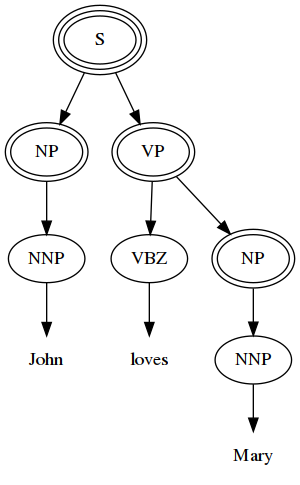
\includegraphics[scale=0.32]{figures/dots/john_agrajz.png}
\caption{A \textit{John loves Mary.} mondat ágrajzon ábrázolva}
\label{fig:john_agrajz}
\end{figure}

Jól látszik , hogy a fa levelei a szavak(\textit{John}, \textit{loves}, \textit{Mary}), amik fölött a szófaji kategóriák (\textit{NNP}, \textit{VBZ}) helyezkednek el, mint unáris csúcsok.
Az \textit{NP}, \textit{VP} a főnévi és igei kifejezéseket jelölik, az \textit{S} pedig a mondat gyökere (az angol \textit{sentence} szó után).


%----------------------------------------------------------------------------
\subsection{Dependenciaelemzés és az UD}
\label{sec:ud}
%----------------------------------------------------------------------------
A dependencia-alapú megközelítés szerint a szintaktikai szerkezet lexikai elemekből áll, amelyeket bináris kapcsolatok kötnek össze. A \texttt{dependencia} fogalma azt jelenti, hogy a szavak (\texttt{fej} és \texttt{dependens}) irányított kapcsolatokkal vannak összekötve.  Általában az állítmány a gráf gyökércsomópontja vagy a strukturális középpontja a mondatnak. A mondat szerkezetét a fejek és dependensek közötti viszonyok adják. Sok jól ismert elmélete van a függőségi nyelvtanoknak, összefoglalásért lásd \cite{Nivre:2005}.

A dependencianyelvtanok általában az információt egy DAO gráfon szemléltetik, amelyek csúcsai a szavak, és élei pedig a szavak közötti viszonyok. Az ilyen függőségi gráfok leírására többféle formalizmus létezik. Az NLP területén a függőségi gráfokat használják legtöbbször a szintaxis reprezentálására. Mi a kutatásunk során az \texttt{UD}-t (Universal Dependencies)\cite{deMarneffe:2014} használtuk.

Az UD projekt egy nyelvek közötti konzisztens annotációs rendszer és fa-adatbázis hatvannál is több nyelvre. Kategóriák és annotációk univerzális készletét nyújtja, miközben megenged nyelvfüggő kiterjesztéseket is. Az UD a Stanford Dependencies-ből \cite{deMarneffe:2008} fejlődött ki, amelyet egyesítettek a Google univerzális címkékkel \cite{Petrov:2011}, az “Interset feature inventory”-nak egy átdolgozott részhalmazával \cite{Zeman:2008} és  a CoNLL-X formátum egy átdolgozott verziójával \cite{Buchholz:2006}. Az UD lehetővé teszi nyelvfüggetlen dependenciaparszerek kiértékelését.

\begin{figure}[h]
\centering 
\xytext{
    \xybarnode{I} 
    &~~~&
    \xybarnode{saw} 
      \xybarconnect(UL,U){-2}"_{\small nsubj}"
      \xybarconnect[18](U,UR){8}"^{\small punct}"
      \xybarconnect[12](UR,UR){6}"^{\small obj}"
    &~~~&
    \xybarnode{the} 
    &~~~&
    \xybarnode{white} 
    &~~~&
    \xybarnode{cat} 
      \xybarconnect[8](U,U){-4}"_{\small det}"
      \xybarconnect(UL,U){-2}"_{\small amod}"
    &~~~&
    \xybarnode{.}
}
\caption{Az \textit{I saw the white cat.} mondat függőségi elemzése}
\label{fig:deptreeEN}  
\end{figure}

\begin{figure}[h]
\centering 
\xytext{
    \xybarnode{A} 
    &~~~&
    \xybarnode{fehér} 
    &~~~&
    \xybarnode{macskát} 
      \xybarconnect[8](U,U){-4}"_{\small det}"
      \xybarconnect (UL,U){-2}"_{\small amod}"
    &~~~&
    \xybarnode{láttam} 
      \xybarconnect(U,UR){-2}"_{\small obj}"
      \xybarconnect(UR,UL){2}"^{\small punct}"
    &~~~&
    \xybarnode{.}
}
\caption{Az \textit{A fehér macskát láttam.} mondat függőségi elemzése}
\label{fig:deptreeHU}  
\end{figure}

Ebből a két példából is jól látszik az UD nyelvfüggetlensége. A mondat angol és magyar verziójában a szavakat megfeleltetve az élek is könnyen megfeleltethetőek.
Itt az élek jelentése a következő:
\begin{itemize}
\item \emph{punct : } 
A feje az állítmány, a dependense pedig a mondatot záró pont vagy más írásjel.
\item \emph{det : } 
A szerkezet fejét a rá vonatkozó névelővel (determinánssal) köti össze. 
Például a \textit{The} a \textit{cat}-nek, és az \textit{a} pedig a \textit{macskát}-nak determinánsa.
\item \emph{amod: } 
Azt jelöli, hogy a fejnek a dependens a mellékknévi módosítója.
Például a \textit{white} a \textit{cat}-et, a \textit{fehér} a \textit{macskát} szót módosítja.
\item \emph{obj : }  
A feje az állítmány, a dependense pedig a tárgy.
Jelen esetben a \textit{cat} vagy a \textit{macskát} a mondat tárgya.
\item \emph{nsubj : } 
Azt jelöli, hogy a fejnek a dependens a névszói alanya. 
Ekkor persze a fej a mondat állítmánya.
Ez azért nem jelenik meg a magyar mondat esetén, mert a magyarban nem vagyunk kötelesek megadni az "én" személyes névmást, mivel az állítmány ragozása jelöli a rejtett alanyt.
\end{itemize}

%----------------------------------------------------------------------------
\section{Szemantika}
\label{sec:semantics}
%----------------------------------------------------------------------------

A szemantika nem foglalkozik a jelek külalakjával és szerkezetével, középpontjában a jelentés áll.
A jelentést viszont nehéz reprezentálni. Azt is nehéz megfogni, hogy az egyes szavak mit jelentenek.
Az NLP-ben számos megközelítés létezik a jelentés reprezentálására. A \texttt{szemantikai elemzés} (semantic parsing) célja, hogy a nyers szövegből, vagy valamely szintaktikai reprezentációból előállítsa a szemantikai reprezentációkat.

Az egyik a szóvektorok. Eszerint a szavak jelentését a környezetében felbukkanó szavak adják.
Pontosabban annak gyakorisága, hogy amikor a szó feltűnik, akkor egyes szavak is megjelennek a környezetében. Ezekből a gyakoriságokból egy szótárnyi hosszú vektor készíthető.
Itt a szavak jelentése nem más, mint egy szótár számosságnyi dimenziós térben a pozíciója.
Itt nem csak hogy a közel azonos jelentésű szavak közel helyezkednek el egymáshoz képest, de egyes összefüggések is kihozhatóak vektor műveletek ként.
Például a \textit{királynő} vektora megkapható a \textit{király} vektorából.
Csak ki kell belőle vonni a \textit{férfi} vektorát és hozzá kell adnunk a \textit{nő} vektorát.
Ugyanakkor ez a módszer csak a szavak jelentését reprezentálja.
 
A másik módszer az irányított gráfok használata.
Itt azt feltételezzük, hogy a szavak mögötti fogalmak és az azok közötti kapcsolatok adják a mondat jelentését.
Ekkor egy gráf csúcsaiban fogalmakkal, és azok között címkézett élekkel reprezentáljuk a jelentést.
Ennek mezei példája például egy mindmap, ahol az egymással asszociatív viszonyban lévő szavakat cimkézetlen élekkel kötjük össze.
Ez a módszer viszont csak a mondattal foglalkozik.
Az már más kérdés, hogy az emberek az adott fogalmakhoz milyen további jelentéseket tárasítanak.
A ~\ref{sec:4lang}. fejezetben tárgyalt \texttt{4lang} is egy ilyen megközelítést alkalmaz.

%----------------------------------------------------------------------------
\subsection{4lang}
\label{sec:4lang}
%----------------------------------------------------------------------------
A \texttt{4lang}  \cite{Kornai:2015} egy formalizmus, ami irányított gráfokat épít szemantikai reprezentáció céljával. A gráfban a csúcsok nem szavakat, hanem nyelvfüggetlen fogalmakat jelölnek. Ezeknek a fogalmaknak már nincsenek nyelvtani jellemzőik és a kompetens beszélők közös tudását reprezentálják a fogalomról. Például a \textit{fagy} mint főnév vagy mint ige, illetve a \textit{fagyás} vagy \textit{fagyott} szavak nincsenek megkülönböztetve a 4lang reprezentációban \cite{Recski:2018}. Ezáltal a 4lang fogalmak és a nekik egy nyelvben megfelelő szavak között egy a többhöz kapcsolat áll fenn.

A csúcsokat háromféle él kapcsolhatja össze:
0-él reprezentálja a tulajdonságokat. Például \textit{$virág -0-> szép$}, az \textit{$IS\_A$} viszony \textit{$virág -0->  növény$} és unáris predikáció \textit{$virág -0-> bimbózás$}.
1 és 2-élek bináris predikációkat kapcsolnak az argumentumaikhoz. Például \textit{$James <-1- szeretet -2> kutya$}.

Létezik egy másik élkonfiguráció is, ami megjelenhet 4lang gráfban, \textit{$w_1 <-0-1-> w_2$} . Erre azért van szükség, hogy konzisztensen lehessen jelölni a tárgy és predikátum közötti viszonyt. Vegyük például a \textit{I’am writing.}(\textit{Én éppen írok})  mondatot az \textit{$i -0> write$} 4lang gráffal és az \textit{I’am writing a letter}(textit{Én egy levelet írok éppen}) mondatot az \textit{$i <-1- write -2-> letter$} gráffal . Ez a két példa a dupla él nélkül azt jelentené, hogy  az \textit{I} és a \textit{write} között attól függ a viszony, hogy adott-e a tárgy vagy sem. \cite{Recski:2018}

A 4lang könyvtár tartalmaz eszközöket, amelyek képesek 4lang gráfokat építeni nyers szövegből és szótári definíciókból (text\_ to\_ 4lang, dict\_ to\_ 4lang). A dep\_ to\_ 4lang 4lang viszonyokat nyer ki szövegből a Stanford Parser \cite{DeMarneffe:2006} kimenetének a feldolgozásával és a Stanford függőségek 4lang részgráfokká való leképezésével.
4lang a neve egy kézzel alkotott  fogalmi szótárnak is, amely négy nyelven tartalmaz több mint 2000 fogalom nyelvfüggetlen definícióját (magyar, angol, latin, lengyel). \cite{Kornai:2013}


%----------------------------------------------------------------------------
\subsection{A 4lang és az UD különbségei}
\label{sec:4LvsUD}
%----------------------------------------------------------------------------
A munkánk során, mint majd alaposabban is bemutatom a nyelvtan generálásánál, alaposan kihasználtuk a 4lang és az UD közötti hasonlóságot. Mindkét esetében egy irányított gráfról beszélünk: a csúcsok megfeleltethetőek a szavaknak, és az élek szavak közötti viszonyokat jelölik. Maguk a függőségek is sok esetben megfeleltethetőek egymásnak. Például a \textit{$w_1 -amod-> w_2$} viszony az UD-ból megfelel a \textit{$w_1 -0-> w_2$} viszonynak a 4lang-ból.

A kettő között ugyanakkor fontos elméleti és jelölésbeli különbségek vannak. Az UD a mondatok szintaxisát reprezentálja, míg a 4lang a szemantikáját (jelentését). Az UD-ben a csúcsok maguk a szavak, míg 4lang-ban a szavaknak megfeleltethető fogalmak. Az UD élei a szavak közötti nyelvtani viszonyt jelölik, a 4lang élek pedig a szavak közötti szemantikai függőségekket. A 4lang élek és az UD függőségek között egy a többhöz viszony áll fenn, ahogy a szavak, és a 4lang beli fogalmak között is. Ez persze azt jelenti, hogy az UD már tartalmazza a szemantikára vonatkozó információkat is, de csak közvetetten.

\begin{table}[h]
    \centering
    \begin{tabular}{lc}
        \toprule
        Függőség & Él \\
        \midrule
        amod & \multirow{7}{*}{\edge{$w_1$}{0}{$w_2$}} \\
        advmod & \\
        npadvmod & \\
        acomp & \\
        dep & \\
        num & \\
        prt & \\
        \midrule
        nsubj & \multirow{4}{*}{\twoedges{$w_1$}{1}{0}{$w_2$}} \\
        csubj & \\
        xsubj & \\
        agent & \\
        \midrule
        dobj & \multirow{6}{*}{\edge{$w_1$}{2}{$w_2$}} \\
        pobj & \\
        nsubjpass & \\
        csubjpass & \\
        pcomp & \\ 
        xcomp & \\
        \midrule
        appos & \twoedges{$w_1$}{0}{0}{$w_2$} \\
        \midrule
        poss & \multirow{2}{*}{$w_2\xleftarrow1$ \texttt{HAS} $\xrightarrow2w_1$} \\
        prep\_of & \\
        \midrule
        tmod & $w_1\xleftarrow1$ \texttt{AT} $\xrightarrow2w_2$ \\
        \midrule
        prep\_with & $w_1\xleftarrow1$ \texttt{INSTRUMENT} $\xrightarrow2w_2$ \\
        \midrule
        prep\_without & $w_1\xleftarrow1$ \texttt{LACK} $\xrightarrow2w_2$ \\
        \midrule
        prep\_P & $w_1\xleftarrow1$ \texttt{P} $\xrightarrow2w_2$ \\
        \bottomrule                         
    \end{tabular}
    \caption{UD függőségek megfeleltetése 4lang részgráfoknak \cite[p. 12.]{Recski:2018}.}
    \label{table:deps}
    \end{table}

Bár a mondat UD gráfjából a 4lang gráfja levezethető, a két formalizmus tartalma mégsem ekvivalens. A 4lang gráfból már nem mindig vezethető le egyértelműen az UD.

\begin{figure}[h]
\centering 
\xytext{
    \xybarnode{The} 
    &~~~&
    \xybarnode{white} 
    &~~~&
    \xybarnode{cats} 
      \xybarconnect[8](U,U){-4}"_{\small det}"
      \xybarconnect (UL,U){-2}"_{\small amod}"
}
\caption{A 'The white cat' függőségi elemzése }
\label{fig:deptreetiny}  
\end{figure}

\begin{figure}[h]
\centering 
\xytext{
    \xybarnode{white} 
    &~~~&
    \xybarnode{cat} 
      \xybarconnect (UL,U){-2}"_{\small 0}"
}
\caption{A 'The white cat' szemantikai elemzése }
\label{fig:deptreetiny}  
\end{figure}

Ezen a példán jól látható, hogy az \textit{amod} él megfeleltethető egy \textit{0} élnek.
Az is megfiggyelhető, hogy a névelő nem jelenik meg a 4lang gráfban, mivel nincsen önálló jelentése.
A \textit{cats} is elveszti a többes számát, mivel fogalommá általánosul.
A szavaknak a \textit{white} és \textit{cat} szavak szófaja sem jelenik meg a 4lang gráfon.
A 4lang gráf nem is alakítható vissza egyértelműen UD gráffá ez elveszett információk miatt.

A többjelentésű szavak is nehezítik a helyzetet, mivel ekkor a szónak megfelelő fogalom már függ a szó környezetétől is.
Sőt egyes esetekben még a környezetből sem határozható meg egyértelműen a szóhoz társuló fogalom. 


%----------------------------------------------------------------------------
\section{A kutatás célja}
\label{sec:goals}
%----------------------------------------------------------------------------


A kutatásunk célja az, hogy a nyers szöveg és a feljebb leírt interpretációk bármelyikéből le tudjuk a többit generálni. Ha az egyik interpretációhoz a másikból több is tartozik, akkor képesek akarunk lenni az összes verziót legenerálni és a legalkalmasabbat automatikusan kiválasztani valószínűségi súlyozás segítségével. Minél kevesebb nyelvet szeretnénk használni, és minél kevesebb módszertant. Ez utóbbi szemponttól azt várjuk, hogy könnyebb lesz a kódot karbantartani és bővíteni további interpretációkkal. Mindezt hatékonyan is szeretnénk csinálni. E téren az alap célunk egy négyzetes lefutási idő a bemenet méretének függvényében. Ezeknek a megkötéseknek az IRTG nyelv eleget tesz, hiszen nagyon eltérő interpretációk esetében is legfeljebb interpretációk száma plusz egy nyelvet kell használnunk. Ugyanakkor, ha kiegészítjük az IRTG-t egy összetettebb gráfalgebrával, az képes lehet minden interpretáció hatékony leírására és mindehhez két nyelvet kellene használnia.

%----------------------------------------------------------------------------
\section{Az IRTG és az alárendelt algebrák}
\label{sec:aists}
%----------------------------------------------------------------------------
Ebben a fejezetben a kutatás során használt környezetről (Alto), formalizmusról (IRTG), algebrákról(SA,TTA,SGA), hátrányaikról és az ezeket kiküszöbölő ideiglenes megoldásainkról lesz szó.


%----------------------------------------------------------------------------
\subsection{Az Alto}
\label{sec:alto}
%----------------------------------------------------------------------------
A kutatás során a kódot az Algebraic Language Toolkit-tel, avagy Alto-val \footnote{\url{https://github.com/coli-saar/alto}} fordítjuk és futtatjuk. Az Alto egy nyílt forrású parszer, ami többféle algebrát is megvalósít, amelyek IRTG-be ágyazva használhatók.
Ezek egyike az s-graph és a tag tree algebra. Ezen kívül is szabadon bővíthető új algebrákkal. Már korábban is használták gráftranszformációra és szemantikai elemzésre is \footnote{\url{https://github.com/kornai/4lang/blob/master/exp/alto/ud/en_ud_bi.irtg}}. Nagy előnyt jelent, hogy Java-ban lett implementálva , így szinte bármely platformon futtatható. Ezen kívül rendelkezik grafikus és konzolos felhasználói felülettel is.


%----------------------------------------------------------------------------
\subsection{Az IRTG}
\label{sec:irtg}
%----------------------------------------------------------------------------
Az IRTG (Interpreted Regular Tree Grammar, interpretált reguláris fa-nyelvtan) \cite{Koller:2011} egy kontextusfüggetlen nyelvtan, ami egy vagy több algebrába beágyazott újraíró szabályokból áll.

\begin{figure}[h]
\begin{verbatim}
NP -> _NP2_amod_JJ_NN(JJ, NN)
[string] *(?1,?2)
[tree] NP2(?1, ?2)
[ud] merge(f_dep(merge("(r<root> :amod (d<dep>))", r_dep(?1))),?2)
[fourlang] merge(f_dep(merge("(r<root> :0 (d<dep>))", r_dep(?1))),?2)
\end{verbatim}
\caption{Egy, az \texttt{amod} relációt leíró IRTG-szabály négy algebrával}
\label{fig:amod_irtg}
\end{figure}

A szabálysorok egy környezetfüggetlen nyelvtan átírási szabályait adják meg. A szabályok feldolgozásakor először egy \texttt{levezetési fa} (derivation tree) épül, amelyek a nonterminálisokat lecserélő szabályokat tartalmazzák. Egy szabályt a következő módon lehet definiálni (a sablonban a változó részeket \{\$ \$\}zárójellel jelöltem, ahol a \$ a Slot kifejezésből ered, a \{\} pedig a nem szöveg elemeket jelöli):
\begin{verbatim}
[{$ interpretáció neve $}] {$ interpretáció lépése $}
\end{verbatim}
A interpretációk nyelve és kimenete többféle is lehet.  Választható például a szöveg kimenetű \texttt{string algebra}, a csúcssorrendet tartó, fa kimenetű \texttt{tag tree algebra}, vagy  az irányított gráf kimenetű \texttt{s-graph algebra}. Az algebrák és az interpretációk között egy a többhöz kapcsolat van. Az interpretációk egymástól teljesen függetlenek. Egy szabályban minden interpretációt meg kell adni. Minden átírás során, minden interpretációra vonatkozó derivációba beszúródnak az alkalmazott szabályban az interpretációhoz tartozó lépések. A beszúrás helyét ?{$  szám $}-ként jelölik minden interpretációban. Itt a szám annak a jobb oldali nemterminálisnak a sorszáma, amely átírása során szúródik be az alkalmazott átírási szabálynak az interpretációhoz tartozó lépése. Az IRTG futtatásakor bármelyik interpretáció lehet a bemenet. Az ALTO a bemeneti interpretáció algebrájának megfelelő formátumú bemenetet vár. A futás során az ALTO keres a bemenethez egy olyan levezetést, ami megfelel a környezetfüggetlen nyelvtannak és a bemenetet adja eredményül. Ezt követően a levezetési fa szerint felépíti a többi interpretációt is, és végrehajtva őket, előállítja a kimeneteket.

Tekintsük az 1.ábrán bemutatott szabályt. Ez a szabály egy melléknévből (adjective, JJ) és egy főnévből(noun, NN) készít egy két gyermekű főnévi kifejezést (noun phrase, NP). A két szó között melléknévi módosítói (adjectival modifier, amod) viszony áll fenn az UD gráfban. Ennek megfelelően neveztük el a szabályt “\_ NP2\_ amod\_ JJ\_ NN”-nek. Az interpretációk sorban a nyers szöveg, a szintaktikai fa, az UD gráf és a 4lang gráf.
Itt minden reprezentációban a “?1” és “?2” az, ahova a “JJ” és “NN” jobb oldali nemterminális szimbólumok átírásánál keletkező kifejezések kerülnek. Ezek az interpretációk bemenetei. Jelen esetben a “?1” a “JJ” és a “?2” az “NN” szimbólum interpretációinak a helye. A két jobb oldali nemterminális kiértékelése után minden interpretációba a vele azonos interpretáció kimenete kerül, stringé a stringbe stb.

A string interpretációhoz a string algebra tartozik. Jelen esetben a bemeneti két szót fűzi össze. A tree interpretációhoz a tag tree algebra tartozik, ami egy “NP2” címkéjű csúcs alá szúrja be a két bemenetet. Ez az algebra állítja elő a szintaktikai fát. A bemenete két-két csúcs.  A negyedik és ötödik sorhoz is az s-graph algebra tartozik. Mindkettő irányított éllel köti össze a két bemenetet. Az UD egy \textit{amod}, a 4lang pedig egy \textit{0} címkéjű éllel. Itt mindkét esetben mindkét bemenet csak egy címkézett csúcs. A nevüknek megfelelő gráfokat állítják elő. Magasabb szintű szabályoknál már az UD és 4lang bemenetek összetett irányított gráfok lesznek. Mi elsősorban az előbb említett három algebrát használjuk, de ezeken kívül más algebra is használható az IRTG nyelvben, mint például a wide string algebra, a tree with arities algebra vagy a set algebra. Ezek nem részei a dolgozat fókuszának.



%----------------------------------------------------------------------------
\subsection{Az SA}
\label{sec:sa}
%----------------------------------------------------------------------------
Az SA (\texttt{string algebra}) kétségtelenül az összes IRTG alatt elérhető algebra közül a legegyszerűbb. Itt csak szövegek konkatenációjára (összefűzésére) van lehetőség. A bemenet és kimenet nem tartalmaz slotokat vagy egyéb nyelvi elemeket. A műveletet a következő formátumban lehet megadni:
\begin{verbatim}
*( {$  szöveg1 $}, {$  szöveg2 $} )
\end{verbatim}

Egymásba is ágyazható több konkatenáció:
\begin{verbatim}
*( {$  szöveg1 $}, *( {$  szöveg2 $}, {$  szöveg3 $} ) )
\end{verbatim}

Például a \textit{*( "Every mouse”, *( “loves”, “cheese.” ) )} kifejezés az \textit{Every mouse loves cheese.}(\textit{“Minden egér szereti a sajtot.}) szöveget adja vissza. Ez a konkatenáció kommutatív és asszociatív.



%----------------------------------------------------------------------------
\subsection{A TTA}
\label{sec:tta}
%----------------------------------------------------------------------------
A TTA (\texttt{tag tree algebra})-nak, mint az SA-nak, csak egy művelete van, a \textit{merge} (egyesítés). A TTA esetében viszont  már a bemenetek nem nyers szövegek, hanem csúcs sorrend tartó fa gráfok. Tartalmazhatnak slot-okat, amiket TTA esetében \textit{hole}-nak(lyuk) nevezünk. A hole-okat ‘*’-gal jelöljük. Nem lehet őket címkékkel vagy más módon megkülönböztetni, sem eltörölni. A gráf csúcsaiba helyezhetőek. Az ilyen slot-okat tartalmazó fákat nevezzük \textit{tag tree}-nek. A TTA merge műveletének két operandusa van. Mindkét operandus egy tag tree. A jobb oldali fát szúrjuk be a bal oldali fa minden hole-jába a merge során. A merge jele a ‘@’ szimbólum, és se nem kommutatív, se nem asszociatív. A fákat zárójelekkel adjuk meg. Egy csúcs közvetlen gyermekeit és az azok alatti részfát a tőle jobb oldali zárójelben kell megadni vesszőkkel elválasztva. Például így írható le a \textit{John loves Mary} (\textit{János szereti Marit.}) mondat szintaktikai fája:

S3( NP1( NNP( John ) ), VP2( VBZ( loves ),  NP1( NNP( Mary ) ) ), .( . ) )

, aminek ez a fa felel meg:

Ugyanez az igei kifejezés, avagy a VP (Verb Phrase) helyén hole-lal:

S3( NP1( NNP( John ) ), *, .( . ) )

A fenti gráfba a VP2 beszúrása merge-dzsel:

@(S3( NP1( NNP( John ) ), *, .( . ) ),  VP2( VBZ( loves ), NP1( NNP( Mary ) ) ) )

Ennek a műveleti fája:

A TTA egy egyszerű, de átlátható és jól kezelhető nyelv. Ugyanakkor nincs arra lehetőség, hogy a jobb oldali gráfot a bal oldali gráfnak csak adott csúcsába szúrjuk be. A bal oldali gráf minden lyukát felhasználjuk a merge művelet során. Ez már a három gyermekű csúcsok esetében is komoly nehézséget jelentett számunkra. Négy gyermekű csúcsok esetében egyenesen ellehetetleníti a két bemenetű szabályok használatát, amikre a hatékonyság végett törekszünk.

Például ha van már egy szavak nélküli:

S3( NP1( * ), VP2( *,  NP1( * ) ), * )

fánk, akkor abból sose leszünk képesek az eredeti:

S3( NP1( NNP( John ) ), VP2( VBZ( loves ),  NP1( NNP( Mary ) ) ), .( . ) )

fát előállítani, mert már az első szóhoz tartozó csúcsok, az “NNP(John)” beszúrása esetén az:

S3( NP1( NNP( John ) ), VP2( NNP( John ),  NP1( NNP( John )) ), NNP( John ) )

fát kapjuk. 
Éppen ezért a interpretációs lépések segítségével kell összerakni szabályról szabályra ezt a fát. 
Lásd példa~\ref{sec:example1}.

Ez a példa is jól mutatja, hogy egy két gyerekű csúcsot, mint a VP2, össze tudunk rakni egy két bemenetű szabályban. Egy három gyerekűt, mint az S3, már nem, hiszen a három gyereket nem tudja mind megkapni egyszerre. Ekkor kénytelenek vagyunk két szabály alatt előállítani a szerkezetet merge használatával. Az ilyen három gyermekű csúcsok gyakoriak a Penn Treebank Szintaktikai Fáiban.  Ilyen a \textit{the black cat} (\textit{a fekete macska}) főnévi kifejezés is, aminek a szintaktikai fája az:

NP3( DT( the ), JJ( black ), NN( cat ) ).

A fát merge nélkül praktikusan csak három bemenetű szabállyal lehetséges implementálni.
Lásd példa~\ref{sec:example2}.

Merge segítségével sokkal optimálisabban is megoldható. Lásd példa~\ref{sec:example3}.

Négy gyermekű főneves kifejezések esetében ez már nem lehetséges. 
Ilyen például a \textit{this British industrial conglomerate} (ez a brit ipari összetömörülés), amihez  a:

NP4( DT( this), JJ( British), JJ( industrial), NN( conglomerate) )

fa tartozik. Ezt a fenti logikával nem tudjuk helyesen megoldani. Lásd példa~\ref{sec:example4}.

Itt a második NP\_BAR elkészítésekor, a merge művelet során a JJ  mindkét lyukba beszúródik, így a: NP4( DT( this), JJ( British), JJ( British), NN( conglomerate) )

Ezt a TTA korlátai miatt nem tudjuk megkerülni.

Négy gyermekű csúcs egy helyes szintaktikai fában nem fordul elő. A középső JJ-k helyes esetben egy ADJP-t alkotnának. Mi a Stanford parser kimenete alapján dolgoztunk, ami sok esetben ilyen fát adott eredményül.


%----------------------------------------------------------------------------
\subsection{Az SGA}
\label{sec:sga}
%----------------------------------------------------------------------------
Az SGA (\texttt{s-graph algebra}) a legbonyolultabb algebra, amit használunk. Több műveletet és összetett gráfnyelvet használ. Az egyetlen hiányossága, hogy nem képes a csúcsok sorrendjét kezelni. Ezért szorulunk a TTA használatára csúcssorrendet tartó fák esetén. Az SGA-ban egy csúcsnak három attribútuma van, \texttt{name} (név), \texttt{tag} (címke) és \texttt{mark} (megjelölés). Ezeket a következő szintaxissal tudjuk megadni: \{\$ name \$\}/\{\$ tag \$\}<\{\$ mark \$\}>. Az attribútumok közül a tag és a mark elhagyható. A név azonosítja a csúcsot adott környezetben, a címke jelenik meg a gráf kirajzolásakor és a jelöléssel hivatkozhatunk a csúcsokra egyes műveletek során. Az éleket :-tal jelölik, és címkézhetőek. Alapesetben az él balról jobbra mutat, de van mód jobbról balra mutató él definiálására is. A gráfokat stringként kell megadni, például a:

“(ROOT :root (loves/loves :nsubj (John/John) :dobj (Mary/Mary) ) )”

a “John Loves Mary.” mondat UD Gráfját írja le, ami így néz ki:
\begin{figure}[h]
\centering
\graphicspath{./}
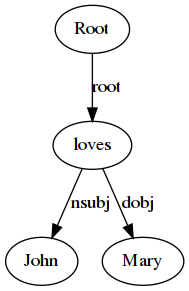
\includegraphics[scale=0.32]{figures/dots/example5_3.png}
\caption{A \textit{John loves Mary.} mondat UD gráfja}
\label{fig:JLM_UD}
\end{figure}


A nyelvtan legfontosabb három művelete a \texttt{forget} (elfelejt), \texttt{rename} (átnevez) és a \texttt{merge} (egyesít). A forget és a rename a jelölések manipulációjára való. A forget művelettel lehet egy jelölést az összes vele megjelölt csúcsról törölni. A rename művelettel egy adott jelölés minden megjelölt csúcson lecserélhető egy másik jelölésre. A merge művelet bemenete az előzőekkel ellentétben két gráf. A bal oldali gráf minden megjelölt csúcsába beszúrja a jobb oldali gráf minden ugyanazzal a jelöléssel megjelölt csúcsát. A műveletek egymásba ágyazhatóak. Csak az egymást követő forget műveletek cserélhetőek fel minden esetben. Forget-et a “f\_ \{\$ jelölés\_ neve \$\}(\{\$ gráf \$\})”
 formában lehet megadni, ahol természetesen a gráf helyén állhat újabb művelet is.  Rename-t pedig a:
\begin{verbatim}
r_{$ régi_jelölés $}_{$ új_jelölés $}( {$ gráf $} )
\end{verbatim}
formátumban lehet megadni. A rename esetén a leváltandó jelölés neve elhagyható és abban az esetben a “root” jelölésű csúcsokon fogja végrehajtani. A merge formátuma hasonlít leginkább a közismert programozási nyelvek függvényhívásaira.: merge(\{\$ gráf1 \$\}, \{\$ gráf2 \$\}) Lásd példa~\ref{sec:example5}.

A példa sok szabálya megfeleltethető a tree reprezentáció esetében használttal. Ennek oka az, hogy a nyelvtanokat úgy írtuk meg, hogy azokat könnyű legyen összeilleszteni. Általában a szintaktikai fa egy csúcsát vagy egy három gyermekű csúcsának a felét rakjuk össze egy szabály alatt, és az UD gráfba kerülő élek és a jobb oldali nemterminális szimbólumok szerint nevezzük el a szabályokat. Mivel az UD gráfban és 4lang gráfban sok a hasonlóság, azt is hozzá adom az egyesített nyelvtan példában. Lásd példa~\ref{sec:example6}.

Az s-graph algebra egy jól használható nyelv, de módosítani és javítani is nehéz. Ennek elsődleges oka a bonyolult szintaxis.

A műveletek nehezen átláthatóak. A legtöbb művelet jele egy-egy betű, és így se nem olyan beszédes, mint az aritmetikai operátorok, se nem olyan felismerhető, mint az SGA merge vagy a TTA ‘@’ jelölése. Az operandusok egy részét is a függvény nevében jelölik.  Ez mind sokat ront az átláthatóságon. Sok esetben fölösleges, hogy külön művelet a forget és a rename a merge-től. Egyszerűbb lenne a merge attribútuma ként megadni, hogy a bal oldali gráfból milyen jelölést párosítunk a jobb oldali gráf melyik jelölésével. Azt is lehetne opcionális operandus, hogy a merge után melyik mark legyen elfelejtve.

Ha már a nyelv célja egyértelműen a tömörség, akkor a merge lehetne \textit{‘@’} a TTA-hoz hasonlóan. A forget és a rename is lehetne pl. \textit{‘\&’}, mint reference, \textit{‘\#’}, \textit{‘\%’} vagy egyszerűen egy \textit{‘R’}, ahol a forget egyszerűen egy olyan rename, ahol az új jelölés hiányzik és nem a régi.

A \textit{':'} semmilyen asszociatív viszonyban nincsen az irányított élekkel. A \textit{‘:’}-ot lehetne például \textit{-\{\$ él\_ címke \$\}-}-re cserélni irányfüggően kacsacsőrökkel a végén.
A csúcsok deklarációjában az attribútumok egymástól teljesen eltérő szintaxissal vannak jelölve teljesen feleslegesen. A csúcsok adatai is mehetnének egy szögletes zárójelbe. A zárójelen belül \textit{[n=\{\$ name \$\} , t=\{\$ tag \$\} , m=\{\$ mark \$\}]}formában egyértelmű is lenne, hogy melyik melyik. Így a sorrendjük lehet cserélhető. Így bármelyikük elhagyható anélkül, hogy zavaróvá válna. Itt attribútumok felsorolásáról van szó, így a kis betű sem zavaró. Adott sorrend mellett a kis betűk is elhagyhatóak:
\begin{verbatim}
[{$ name $} | {$ tag $} | {$ mark $}].
\end{verbatim}
 Lásd példa~\ref{sec:example7}.

Véleményem szerint ez sokkal tisztább módja lenne és tördelni is sokkal egyszerűbb. Ha az egyik forget vagy rename műveletetre nincs szükség, akkor csak elhagyjuk a hozzá tartozó attribútumokat . Még ennél is szebb lenne, ha a műveleteket operációs jelek jelölnék. Lásd példa~\ref{sec:example8}.

Ugyanakkor ez már túlzottan eltér a gráfleíró nyelvek hagyományos stílusától, és tördelni is nehézkesebb. Operátoros esetben pedig szükség lenne egy sorrendiségre is, ami nem lenne mindenki számára triviális. Arról nem is beszélve, hogy a rename művelet három bemenetű, így nem lehet egy operátorral elvégezni, ahogy az összetett merge négy operátorát is erőltetetten hat.


%----------------------------------------------------------------------------
\section{Az IRTG és az ALTO hiányosságai}
\label{sec:shortcomming}
%----------------------------------------------------------------------------
Mivel a szakdogám célja az IRTG nyelv fejlesztése, ezért ebben a fejezetben az IRTG és az ALTO hiányosságairól kívánok részletes áttekintést nyújtani.
Arra is ki kívánok térni, hogy hogyan lehetett volna, és lehetne az ezek által okozott problémákat megoldani.
Először az IRTG-ről lesz szó, majd az LATO-val folytatom.

%----------------------------------------------------------------------------
\subsection{Az IRTG hiányosságai}
\label{sec:IRTGshortcomming}
%----------------------------------------------------------------------------

Az IRTG nem egy programozási nyelv, hanem egy nyelvtan. A szabályok egymás alatt adhatóak meg és csak backspace karakterekkel és kommentekkel tagolhatóak. Egy nyelvtan több fájlra nem szedhető szét. A fájl elején fel kell sorolni az interpretációkat, és egyik interpretáció sem hagyható el egyik szabályból sem, még akkor sem, ha semmit sem adnak vissza. A kutatás során egy olyan nyelvtant készítettünk, ami 2700 szabályból áll és négy interpretációból. Ez ha a szabályokat üres sorokkal választjuk el, akkor 16204 sor kódot jelent egyetlen fájlban. Egy ekkora kódot nehéz karbantartani, átlátni, fejleszteni. Tehát szükség van IRTG-ben az importálásra.


Rengeteg esetben a szabályok alig egy-egy szóban térnek el. Lásd példa~\ref{sec:example6}.
Itt a \textit{John} és a \textit{Mary} szóhoz tartozó terminális szabályok között csupán maguk a szavak jelentik a különbséget. A string interpretációban is csak maga a szó jelenik meg. Más szófajú szavak esetében is csak a szabály sort és tree reprezentációt kell még módosítani. Az ilyen esetek miatt nagy kár, hogy az IRTG-ben nem lehet szabályokat egymásból vagy egy közös ősből származtatni.


Sokszor egy szó szófaja egy másik szófaj alkategóriája. Ilyen például az NNP (proper noun, tulajdonnév), ami az N (noun, főnév) alketegórája. Az egy főkategóriába tartozó szófajok sok esetben ugyanúgy viselkednek. Például egy NP-ben, ami egy N-ből és egy JJ-ből áll, minden esetben a két szó között egy amod él lesz az UD gráfban. Ugyanakkor vannak olyan esetek is, amikor az alkategóriáknak csak egy részhalmaza viselkedik hasonlóan. Egy alkategória esetében kétféleképpen lehet megoldani ezt. Az egyik verzióban általánosítunk, tehát az alkategóriákat ugyanúgy kezeljük. Ekkor jelentős áldozatot hozunk a pontosság terén. Más esetben minden egyes alfajra előállítunk minden szabályt, amivel előfordul. Ekkor jelentős áldozatot hozunk hatékonyság terén, mivel sokkal több szabályon kell végigiterálnia az ALTO-nak az IRTG futtatásakor. Erre jó megoldás lenne, ha egy szabálysorban minden olyan nemterminális szimbólumot meg tudnánk adni, amire a szabálynak minden interpretációhoz ugyanaz a lépés tartozik. Erre jó megoldás lenne, ha a szabálysorban regexszel lehetne megadni mindegyik jobb oldali nemterminális szimbólumot.


Az IRTG szabályokban mindenre más és más algebrát használunk más és más nyelvvel. Ennek az az oka, hogy mint már az algebráknál részleteztem, minden algebrának vannak hiányosságai. Az IRTG maga lehet önmagában átlátható, de ha az algebrái sokfélék, és némelyiket önmagában is nehéz átlátni, akkor az az IRTG-re is közvetlen hatással lesz (lásd s-graph algebra). Hiába a sokféleség, ha egyes feladatokra csak egy olyan algebra létezik, ami megfelel a célnak és az is erősen korlátozott. Egy algebrára van csak szükség. Egy olyan algebrára, ami az s-graph algebra szintjén van, de átlátható és képes mint a csúcsok sorrendjét kezelni, mint a címkék konkatenációját. Elvégre a szöveg is kezelhető egyetlen csúcs ként. Egy ilyen algebrában az is fontos, hogy ne kelljen az egyszerű műveleteket sokkal terjedelmesebben megoldani, mint ha azt az egyszerű algebrákkal végeznénk. Az s-graph javítására az algebra kapcsán mutattam példát, de egy ilyen univerzális algebra már szemantikai változtatásokat is igényelne.


Gyakori az IRTG-ben az, hogy kulcsszavak ütköznek pár változónak a nevével, ami felesleges errort okoz a feldolgozás során. Például az \textit{interpretation} szóhoz generált terminális szabályunk ütközött az interpretation szóval, amivel kezdődnek az IRTG fájlok elején az interpretációkat definiáló sorok. Ha a szabálynak így kezdődik a neve, akkor már nem fogadja el a futtatókörnyezet. Erre a legegyszerűbb megoldás az, ha a nyelvben megjelenik a szöktetés, vagy a kulcsszavakat úgy módosítjuk, hogy ritka speciális karaktereket is tartalmazzanak. Például, ha az \textit{interpretation} helyett \textit{<interpretation>} lenne a kulcsszó. Persze a prőblémát az is megoldaná, ha az ALTO lexerje kellően inteligens lenne a pozíció függő tokenezéshez.

%----------------------------------------------------------------------------
\subsection{Az ALTO hiányosságai}
\label{sec:ALTOshortcomming}
%----------------------------------------------------------------------------

Az ALTO működése iteratív. Végigiterál az összes lehetséges levezetési fán a környezetfüggetlen nyelvtanban, és kiválogatja a bemenetre illeszkedőeket. Ez alatt persze különböző módszerekkel igyekszik elkerülni azokat a lehetséges levezetéseket, amiről már tudja, hogy biztos rosszak lesznek. Erre az egyik legegyszerűbb módszer az, ha a levezetési fákat fentről lefelé generáljuk és kihagyjuk azokat a lehetőségeket, amik már magasabb szinten olyan élet vagy csúcsot vagy azok olyan halmazát vesznek be a derivációba, ami a bemenetben nem szerepel. Ezt hívják \textit{optimalizált DFS Parsing}-nak

Az elvi működés és a megvalósítás következtében az ALTO rendkívül lassú. A feljebb említett 2700 szabályos és négy interpretációs nyelvtan $10^5$ nagyságrendű adaton nagyjából 30 óráig futott, pedig a rendelkezésünkre álló tanszéki szerveren futtattuk. Ez a mi feladatunk esetében elfogadhatatlan. Ezért nem ártana egy hatékonyabb C++ verzió az ilyen méretű munkákhoz. Ma már a C++17 és a hamarosan érkező C++20 is kényelmes programozási nyelv, és nem nagy ördöngösség az alap platformokon futtatható verziókat legenerálni a nyílt forráskódból. Egy könyvtár formájában pythonból is elérhető lenne ez a verzió.

Az ALTO rengeteg felesleges munkát végez, mivel azokat a megoldásokat is kigenerálja a bemenetből, ami más interpretációk derivációjában errorhoz vezet. Az ilyen eseteket is ki lehetne szűrni már a derivációs fa magasabb szintjének az iterációja során. Persze ez debuggolás szempontjából káros, mivel az ilyen esetek kiszámítása nélkül nem tudjuk megfejteni, hogy mi okozta a hibát, de mérvadó méretű adatot nem is akkor fogunk futtatni. Jó lenne, ha ez opció ként lenne elérhető.

Az ALTO mindennek ellenére a jelenlegi legfejlettebb program az IRTG futtatására, és állandó fejlesztés alatt áll. A pontos működését még nem ismerjük. A módosítások többsége viszont a belső működés alapos átdolgozását igényli. Erre jelenleg még nincs erőforrásunk.

%----------------------------------------------------------------------------
\section{Jelenlegi megoldások}
\label{sec:solutions}
%----------------------------------------------------------------------------
A kutatás során az IRTG-t illető problémák többségét kód generálás segítségével küszöböltük ki. Két implementáció készült python nyelven, amik bemeneti adatokból generáltak irtg szabályokat. Kezdetben csak NP-k feldolgozása volt a cél, majd onnan terjesztettük ki az implementációkat VP-k és ADJP-k re. A generátor kódos megoldások legfőbb hátránya a fejlesztőhöz kötöttség volt. Nem tudtunk többen párhuzamosan fejleszteni, mert egyikünk sem értette a másik megoldását kellő mélységben.
Mindkét megoldás a Pann Tree bank szintaktikai fáit és az abból a Stanford Parserral kapott UD gráfokat kapja bemenet ként, amiket python scriptekkel készítettünk elő . Ezek a scriptek végezték a fákból a megfelelő kifejezések részfáinak a kiszedését, a részfák rendezését típus szerint és a fák UD gráfjainak a generálását a Stanford Parserrel.


%----------------------------------------------------------------------------
\subsection{első generátor}
\label{sec:generator1}
%----------------------------------------------------------------------------
Az első generátort én készítettem el 2018 augusztusában. Ez egy objektumorientált megoldás volt. Képes volt kommenteket is generálni, kezelni a rövidítéseket és könnyen bővíthető volt. Ugyanakkor rush development során keletkezett a szakmai gyakorlatom végén, így a kód még nincsen se letisztázva, se alaposan dokumentálva.

Külön osztályban tárolta a nyers szöveg szavait, a fát és az UD-t, majd ezeket rendezte egy közös osztályba. A közös osztály a Data, a nyers szövegé a Terminal, a fáé a Tree, az UD-é és a 4lang-é a Dependency. Az összes osztály rendelkezett saját szöveg bemenetű konstruktorral, ami közvetlen a bemeneti adatok formátumából inicializálja az osztájt.

A Terminal egy szót tárolt és annak a szófaját. A Tree tartalmazta a részfát a Stanford parser formátumában, a TTA formátumában, a TTA formátumában levelek nélkül és külön a szavakat. A Tree legtöbb formátuma csak a kommentek generálásához volt hasznos, de ideiglenesen mindegyiket generálta a program a kommentek végleges formátumától függetlenül. A Dependency tárolta a fej-szót, a dependens-szót, az él UD típusát és az él 4lang típusát. Az UD él 4lang-ra vetítését a Fourlang enum és egy dictionary segítségével végezte. Mint korábban említettem, a szavak és 4lang fogalmak megfeleltetésével még mai napig sem foglalkozunk, de az is ebbe az osztályba került volna és feltételezhetően szintén egy dictionary és enum segítségével.

A generálás innentől szövegkonkatenációból áll az adatok függvényében.
A kifejezés generátor függvények először betöltötték az adatokat a Data osztályokba, majd kiszűrte az egyedi adatokat a levél nélküli fák és UD élek alapján. A komment első sorát aszerint generálta, hogy van-e kapcsolat a szavak között, és hogy a fej vagy a dependens van-e  előrébb. Ez a sor azt írta le, hogy milyen kifejezést milyen típusú szavakból épít a szabály és, hogy a dependens milyen szerepet lát el a mondatban. Ehhez az adatok rövidítéseit a Short2Long osztály segítségével oldotta fel, aminek a betöltendő adatai  a viszonylag kevés szófaj- és éltípus okán kézzel készültek. A következő két komment a szintaktikai fa első példányát tartalmazta a TTA és Stanford Parser formátumában. 

A szabálysort az adatokból nem volt nehéz legenerálni, mivel a szabályok neveit eredetileg is a bemenetek TT interpretációjának gyökere és az UD élek alapján képeztük. A string és tree sorok csak a szabály bal oldali nemterminális szimbólumától függenek, így azok konstans szövegek voltak. Az UD-nél a szövegbe csak az él nevét kellett beszúrni attól függően más sablonba, hogy a csúcsok között van-e kapcsolat, megjelenik-e mindkettő az UD gráfban (a \textit{the},\textit{a} és \textit{an} szavak például nem), és hogy ha van köztük kapcsolat, akkor melyik a fej. A fourlangnak ezek a tulajdonságok már bele voltak kódolva az enum alapú típusába, így itt csak egy else-if ágazaton kellett végigmenni (mivel pythonban nincsen switch case).

Már itt is látszott, hogy számos lehetőség van optimalizációra. Például a kódba ágyazott adatokat is ki lehetett volna szervezni txt fájlokba. Így a fourlang if-else ágai is megoldhatóak lettek volna egy dictionary-vel és karbantarthatóbbak lettek volna az adatok. A kettő magas kifejezések részfái között rengeteg volt a hasonlóság, így könnyedén össze lehetett volna a generáló függvényeiket vonni. A magasabb kifejezés részfákat se lett volna sokkal nehezebb ugyanabban a függvényben generálni. Az adatok feldolgozását és tárolását egy osztályban is meg lehetett volna oldani, ha a bemeneti adatok egy közös fájlban vannak. A nagyon sokadlagos adatokat, mint a fák stanford és 4lang formátuma, nem kellett volna eltárolni. Elég lett volna, ha a többi adatból származtató függvényeket is tartalmazza az egy darab Data osztály. Ezzel azt a duplikációt is elkerülhettük volna hátrány nélkül, hogy a terminálisokat majdnem mindegyik adatstruktúra eltárolta.

Végeredményben viszont még ekkor is egy olyan programunk lett volna, ami az IRTG kódot csak generálja. Végső soron template-elést használt volna, de az IRTG nyelvhez kötött szinten. Az új szabály egyre több kódot jelentett volna, és nehéz lett volna a hibákat meghatározni bárkinek, aki nem dolgozott a program elkészítésén és nem tanulmányozta hosszabb távon.


%----------------------------------------------------------------------------
\subsection{második generátor}
\label{sec:generator2}
%----------------------------------------------------------------------------
A második generátort Ács Evelin kezdte el fejleszteni 2018 őszén.
Ez az első generátortól teljesen függetlenül készült.
Ennek oka, hogy a dokumentálás hiányában nem látták át az első generátor működését.
Ekkor én sem dolgoztam már a projektben, hogy orvosoljam a problémát.
A generátor vívmánya, hogy a bemeneti adatokat gráf ként kezeli, nem pedig egyszerű szöveg ként.
Már ez a megoldás is első sorban sablonolást használ a szabályok előállítására.

Ebben a verzióban a kommentelés és tagolás a legnagyobb hiányosság. 
Bár a projekt jelenlegi tagjai jól átlátják a szabályokat, a szükséges háttér nélkül nehéz a 2700 szabály között eligazodni. 
Ezt persze nem lenne nehéz megoldani, mivel a szükséges adatok már rendelkezésre állnak. 
Ha a szabályokat a baloldali szimbólum szerint és a közös ős fokszáma szerint csoportosítjuk, akkor a tagolás sem nehézkes. 
Persze itt is a Merge és a BAR szabályok (a trenáris csúcsokelkészítésének két lépését megvalósító szabályok) külön kategóriát képeznének. 
A szabályok jelenleg gyakoriság szerint vannak sorba rendezve de a név szerinti sorba rendezés is sokat segítene. 
A kategóriákat mélység szerint is több főkategóriába lehet rendezni.

A kódot persze legtöbben itt sem látjuk át, mivel még részletes dokumentáció nem készült természetesen.
Elvégre a fejlesztés jelenleg is folyamatban van. 
A Slime első verziója nem lesz képes ilyen gráf műveletekre, de könnyű lesz benne olyan kódot készíteni, ami mindenki számára érthető.
Ennek persze az IRTG és a Slime szintaxisának ismerete alapfeltétel. 
Mindezt pedig minimális overhead-del, így csak a bemeneti adatokat szükséges generálni hozzá. 
Mivel az alkategóriákon belül a legtöbb szabály összevonható lesz REGEX és templatelés segítségével, a sorrend sem jelent majd problémát.
Jelenleg úgy tűnik, hogy a teljesen hatékony megoldás a Slime és a második generátor kombinációja.